\documentclass{beamer}
\usepackage{TimosThesePresentation}
\usepackage{TimosTheseCommands}
\usepackage{TimosTheseInfo}


\title[\authorname{} M.Sc. Presentation]{A System for measuring Temperature dependent Surface Photovoltage}

\subtitle{by Timo Bretten}

\institute[\univname]{\univname}

\date[December 10th 2015]{M.Sc. Final Presentation December 10th 2015}

\begin{document}
\begin{frame}
  \titlepage
\end{frame}

\begin{frame}
  \frametitle{Outline}
  \tableofcontents
\end{frame}

\section{Introduction}

\begin{frame}
\frametitle{Some background\dots}
\begin{block}{\dots about my M.Sc. project}
\begin{minipage}{0.55\linewidth}
	\begin{itemize}
		\item Research carried out in 13/14 at \deptname{}
		\item Project had two parts: enhancing solar cells \& setting up a new experimental system
		\item Only part two will be presented
	\end{itemize}
\end{minipage}
\hfill
\begin{minipage}{0.4\linewidth}
\centering
	\includegraphics[width=1\linewidth]{./figs/logos/weiz}
\end{minipage}
\end{block}\end{frame}

\begin{frame}
\frametitle{Motivation}
\begin{block}{The goal of this project is to\dots}
	\begin{itemize}
		\item Use a new experimental Kelvin Probe (\kp{}) system
		\item Add illumination to \enhyphen{new} \kp{}
		\item Compare results from \enhyphen{new} \kp{} to established, \enhyphen{old} \kp{}s
		\begin{itemize}
			\item[$\rightarrow$] Does \enhyphen{old} \& \enhyphen{new} Contact Potential Difference (\cpd{}) agree?
			\item[$\rightarrow$] Does \enhyphen{old} \& \enhyphen{new} Surface Photovoltage (\spv{}) agree?
		\end{itemize}
		\item Ultimately measure temperature dependent Surface Photovoltage (\spv{}(T)) with the new system
	\end{itemize}
\end{block}\end{frame}

\section{Theory}
\begin{frame}
\frametitle{The Contact Potential Difference (\cpd{})}
\begin{block}{Physical Causes of \cpd{}}
\centering
\begin{minipage}{0.4\linewidth}
\centering
	The \cpd{} is the difference in local vacuum levels, here defined as:\\[10pt]
	$\cpd{} \equiv \wfp - \wfs$, \\
	where $\upvarphi$ is Work function\\
\end{minipage}
\hfill
\begin{minipage}{0.55\linewidth}
\centering
	\only<1>{Semiconductor-Metal:\\\includegraphics[width=1\linewidth]{./figs/pres/CPDsemi1}\\\textcolor{RUred}{[1]}}
	\only<2>{Semiconductor-Metal:\\\includegraphics[width=1\linewidth]{./figs/pres/CPDsemi2}\\\textcolor{RUred}{[1]}}
	\only<3>{Semiconductor-Metal:\\\includegraphics[width=1\linewidth]{./figs/pres/CPDsemi3}\\\textcolor{RUred}{[1]}}
	%Figure defining Wf S
	
	%Cite Kronik Shapira
\end{minipage}
\end{block}\end{frame}


\begin{frame}
\frametitle{The Contact Potential Difference (\cpd{})}
\begin{block}{Measuring \cpd{}: The Kelvin Probe (\kp{})}
\centering
\begin{minipage}{0.45\linewidth}
\centering
$\begin{array}{l c c l}
I(t) 	=& \frac{dQ}{dt}	&=& (\cpd{}+V_b) \frac{dC}{dt}	\\
		& 				& &								\\
I(t)		=& 0				&\text{iff}&	V_b=-\cpd{}			\end{array}$
\end{minipage}
\hfill
\begin{minipage}{0.5\linewidth}
\centering
	\includegraphics[width=1\linewidth]{./figs/pres/simple-kp-scheme}\\
	%Equivalent Circuit
\end{minipage}
\end{block}\end{frame}

\begin{frame}
\frametitle{Physical Causes of Surface Photovoltage (\spv{})}
\begin{block}{\spv{}: \cpd{} in the dark dark vs. light}
\centering
\begin{minipage}{0.38\linewidth}
\centering
Different surface potentials in light and dark yield \spv{}:\\[12pt]
$\begin{array}{l l}
\text{\spv} &\equiv \cpd_{\text{l}} - \cpd_{\text{d}}\\
			&\equiv \upvarphi _{\text{s,d}} - \upvarphi _{\text{s,l}}\\
\text{\spv}_{\text{n}} 	&> 0	 \\
\text{\spv}_{\text{p}} 	&< 0			\end{array}$
\end{minipage}
\begin{minipage}{0.6\linewidth}
\includegraphics[width=1\linewidth]{./figs/pres/spvdef}
\end{minipage}
\end{block}\end{frame}

\section{The Systems}
\begin{frame}
\frametitle{Established, \enhyphen{old} \kp{} Systems}
\begin{block}{Ambient \& Glovebox \kp{}s}
\centering
\begin{minipage}{0.55\linewidth}
\centering
\begin{itemize}
	\item Besocke \kp{} head \& controller
	\item Humidity controlled ambient
	\item Glovebox ($<\num{5}$ppm \oxy{} \& \water{})
	\item Xenon lamp \& VariAC ($\sim$\SI{80}{\watt})
	\item Illumination is source of heat!
\end{itemize}
\end{minipage}
\hfill
\begin{minipage}{0.4\linewidth}
\centering
	\includegraphics[width=1\linewidth]{./figs/pres/besocke}\\
	\textcolor{RUred}{[2]}
\end{minipage}
\end{block}\end{frame}

\begin{frame}
\frametitle{\enhyphen{New} System: Cryostat with a \kp{}}
\begin{block}{Lakeshore Cryostat with \McA{} \kp{} \& \led{} illumination}
\centering
\begin{minipage}{0.45\linewidth}
\centering
	\includegraphics[width=1\linewidth]{./figs/pres/Config_TTPX}
\end{minipage}
\hfill
\begin{minipage}{0.45\linewidth}
\centering
	\includegraphics[width=1\linewidth]{./figs/pres/ledspec}
\end{minipage}\\
\hspace{0.25\linewidth}\textcolor{RUred}{[3]}\hfill\textcolor{RUred}{[4]}\hspace{0.2\linewidth}
\end{block}\end{frame}

\section{Experimental}
\begin{frame}
\frametitle{Checking against Established Systems}
\begin{block}{Behaviour at Room Temperature}
\centering
\begin{minipage}{0.45\linewidth}
\centering
	\includegraphics[width=1\linewidth]{./figs/pres/HOPGMcA}
\end{minipage}
\hfill
\begin{minipage}{0.45\linewidth}
\centering
	\includegraphics[width=1\linewidth]{./figs/pres/Sih}
\end{minipage}\\[5pt]\hrulefill\\
\enhyphen{Jumps} probably due to movement of probe head\\
Excellent agreement between systems
\end{block}\end{frame}


\begin{frame}
\frametitle{Checking against Established Systems}
\begin{block}{Behaviour at lower temperatures and \spv{}}
\centering
\begin{minipage}{0.4\linewidth}
\centering
\SI{30}{\nano\metre} AlO$_3$ on Si,\\ 
by plasma-enhanced atomic layer deposition \textcolor{RUred}{[5]}
	\begin{itemize}
		\item $\upvarphi_{\text{Si/Alumina}}$ at \SI{300}{\kelvin}: \SI{4.42+-0.03}{\electronvolt}
		\item $\upvarphi_{\text{Si/Alumina}}$ at \SI{250}{\kelvin}: \SI{4.44+-0.04}{\electronvolt}
	\end{itemize}
\end{minipage}
\hfill
\begin{minipage}{0.55\linewidth}
\centering
\vspace{5pt}
	\includegraphics[width=0.9\linewidth]{./figs/pres/currentseries}
\end{minipage}\\[5pt]\hrulefill\\
Probably no ice, even on very hydrophilic surface\\
\spv{} $\sim$\SI{12}{\percent} too low compared to other system and literature (\textcolor{RUred}{[5]}). Shadows on the sample?
\end{block}\end{frame}

\begin{frame}
\frametitle{Intermission: Choosing a Model System for \spv{}(T)}
\begin{block}{Metal Insulator (MI) Transition in \vadiox{}}
\begin{minipage}{0.6\linewidth}
	\begin{itemize}
		\item metal at $T>T_{MI}$
		\item semiconductor at $T<T_{MI}$
		\item insulator at $T \ll T_{MI}$
		\item $\phantom{\Delta}T_{MI}\approx \phantom{-}\SI{270}{\kelvin}$ \hspace{0.15cm} \textcolor{RUred}{[6]} (W-doped)
		\item $\phantom{\Delta}\upvarphi\phantom{_{MI}} \approx  \phantom{-}\SI{5.15}{\electronvolt}$ \textcolor{RUred}{[7]} (at RT)
		\item $\Delta\upvarphi_{MI} \approx  -\SI{0.15}{\electronvolt}$ \textcolor{RUred}{[7]}
		\item $\Delta\upvarphi_{MI} \approx  \phantom{-}\SI{0.45}{\electronvolt}$ \textcolor{RUred}{[8]} (W-doped)
	\end{itemize}
\end{minipage}
\hfill
\begin{minipage}{0.35\linewidth}
\centering
	\includegraphics[width=1\linewidth]{./figs/pres/vo2gapopening}\\
	\textcolor{RUred}{[9]}
\end{minipage}
\end{block}\end{frame}

\begin{frame}
\frametitle{Temperature Dependent \cpd{} in \wvadiox{}}
\begin{block}{Two independent Measurements: Sweep and Stabilise}
\centering
{\tiny Samples supplied by M. Nakano, RKIEN}\\[-10pt]\hrulefill\\[2pt]
\begin{minipage}{0.45\linewidth}
\centering
	\includegraphics[width=1\linewidth]{./figs/pres/vox1pres}
\end{minipage}
\hfill
\begin{minipage}{0.45\linewidth}
\centering
	\includegraphics[width=1\linewidth]{./figs/pres/vox2pres}
\end{minipage}\\[5pt]\hrulefill\\
Curious behaviour in the range \SIrange{120}{160}{\kelvin}, far below $T_{MI}$ \\
Effect of substrate?
\end{block}\end{frame}

\begin{frame}
\frametitle{Temperature Dependent \spv{} in \wvadiox{}}
\begin{block}{$\rho$(T) and \spv{}(T)}
\centering
\begin{minipage}{0.45\linewidth}
\centering
	\includegraphics[width=0.9\linewidth]{./figs/pres/vo2resis}\\
	{\tiny Measurement by Nir Kedem}
\end{minipage}
\hfill
\begin{minipage}{0.45\linewidth}
\centering
	\includegraphics[width=0.9\linewidth]{./figs/pres/vox3}\\
\end{minipage}\\[2pt]\hrulefill\\[2pt]
$\rho$(T) magnitude and $T_{MI}$-range agrees with literature (\textcolor{RUred}{[7]},\textcolor{RUred}{[10]})\\
$\Delta \upvarphi _{MI}$ observed before; direction \& magnitude unclear (\textcolor{RUred}{[6]},\textcolor{RUred}{[8]})\\
Gradual gap opening process $\rightarrow$ appearance of \spv{}\\
Sign of \spv{} identifies sample as n-type $\rightarrow$ W-doping
\end{block}\end{frame}

\section{Discussion \& Conclusion}
\begin{frame}
\frametitle{Discussion \& Conclusion}
\begin{block}{We showed that\dots}
\centering
\begin{itemize}
	\item \cpd{} is in excellent agreement with established systems
	\item \spv{} $\sim$\SI{12}{\percent} too low. Shadowing?
	\item \cpd{}(T) reproducible and interesting
	\item \cpd{}(T) \& \spv{}(T) reasonable
	\item[$\rightarrow$] Lakeshore + \McA{} + \led{} is a viable experimental system for \spv{}(T)
	\item System has successfully been used in that configuration since 2014, publication forthcoming \textcolor{RUred}{[11]}
\end{itemize}
\end{block}\end{frame}

\begin{frame}
\frametitle{List of References}
\begin{block}{Literature and links}
\centering
	\begin{tabular}{r l}
	\textcolor{RUred}{[1]} & L. Kronik \& Y. Shapira \emph{Surf. Sci. Rep.}, \textbf{37(1-5)}, 1999\\
	\textcolor{RUred}{[2]} & \href{http://www.besocke-delta-phi.de/kelvin.htm}{Besocke Website} \\
	\textcolor{RUred}{[3]} & \href{http://lakeshore.com/products/cryogenic-probe-stations/model-ttpx-cryogenic-probe-station/pages/Overview.aspx}{Lakeshore Website}\\
	\textcolor{RUred}{[4]} & \href{http://www.ledengin.com/files/products/LZP/LZP-00CW0R.pdf}{LEDengin Website}\\
	\textcolor{RUred}{[5]} & D. Cahen~\etal{} \emph{Appl. Phys. Lett.}, \textbf{101}, 2012\\
	\textcolor{RUred}{[6]} & K. Shibuya~\etal{} \emph{Phys Rev. B}, \textbf{82(20)}, 2010 \\
	\textcolor{RUred}{[7]} & C. Ko~\etal{} \emph{ACS Appl. Mater. Interfaces}, \textbf{3(9)}, 2011\\
	\textcolor{RUred}{[8]} & H. Yin~\etal{} \emph{ACS Appl. Mater. Interfaces}, \textbf{3(6)}, 2011 \\
	\textcolor{RUred}{[9]} & M. Nakano~\etal{} \emph{Nature}, \textbf{487(7408)}, 2012 \\
	\textcolor{RUred}{[10]} & K. Shibuya~\etal{} \emph{Appl. Phys. Lett.}, \textbf{96}, 2010 \\
	\textcolor{RUred}{[11]} & D. Cahen~\etal{} \emph{J. Phys. Chem. Lett.}, forthcoming \\
	\end{tabular}
\end{block}\end{frame}


\begin{frame}
\frametitle{Acknowledgements}
\begin{block}{Thanks! to\dots}
\centering
	\begin{tabular}{r l}
	\textcolor{RUred}{Prof. David Cahen} & for his supervision \\
	\textcolor{RUred}{Dr. Hugo Meekes} & for his spontaneous support \\
	\textcolor{RUred}{Igal Levine} & for keeping me (somewhat) on track \\
	\textcolor{RUred}{Nir Kedem} & for always having an answer
	\end{tabular}
\end{block}\end{frame}
\end{document}